\chapter{Метод Виолы-Джонса}

Метод Виолы---Джонса --- алгоритм, позволяющий обнаруживать и распознавать лица на изображениях и видеопоследовательностях в режиме реального времени ~\cite{viola}. Данный метод основан на использовании следующих принципов:
\begin{enumerate}[label=\arabic*.]
    \item Интегральное представление изображения

    Представим исходное изображение в виде матрицы, каждый элемент которой содержит значение интенсивности пикселя. Интегральное представление изображения формируется путем создания новой матрицы, размерность которой совпадает с матрицей исходного изображения. В каждом элементе данной матрицы хранится сумма интенсивностей всех пикселей исходного изображения, находящихся левее и выше текущего пикселя в исходной матрице ~\cite{tomsk}, т. е. элементы новой матрицы рассчитываются по следующей формуле:
    
    \begin{equation}
        L(x,y) = \sum_{i=0, j=0}^{i<=x, j<=y} I(i,j),
    \end{equation}

    где $I(i, j)$ --- значение элемента матрицы исходного изображения, $L(x,y)$ --- значение элемента матрицы интегрального изображения.

    Особенностью интегрального представления является возможность вычисления суммы интенсивностей пикселей внутри произвольных прямоугольных областей ~\cite{tomsk}. Рассмотрим следующий пример, где искомой областью является прямоугольник $ABCD$:

    \begin{figure}[h]
	\centering
	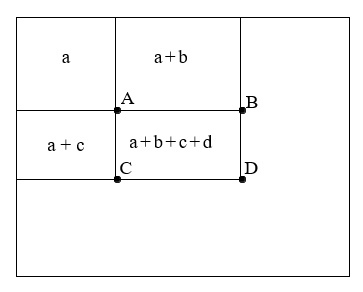
\includegraphics[height=0.25\textheight]{img/integral.jpg}
	\caption{Расчет суммы интенсивностей пикселей в прямоугольнике $ABCD$}
    \label{img:integral}
    \end{figure}

    Сумма интенсивностей пикселей, лежащих внутри области $ABCD$, будет вычисляться по следующей формуле:

    \begin{equation}
        F(ABCD) = F(A) + F(D) - F(B) - F(C),
    \end{equation}

    где $F(X)$ --- суммы интенсивностей пикселей внутри прямоугольной области X.

    Таким образом, для вычисления суммы интенсивностей пикселей внутри произвольных прямоугольных областей требуется четыре обращения к матрице интегрального представления изображения.
    
    \item Признаки Хаара

    Для выделения областей изображения, которые наиболее вероятно содержат нужные объекты, используются признаки Хаара. Признак Хаара --- результат сравнения смежных прямоугольных областей изображения путем вычисления разности сумм интенсивностей пикселей соответствующих прямоугольников ~\cite{novosibirsk}. 
    В методе Виолы---Джонса используются три вида данных признаков: <<два прямоугольника>>, <<три прямоугольника>>, <<четыре прямоугольника>> ~\cite{viola} (рис.~\ref{img:haar} ~\cite{astrahan}).

    \begin{figure}[h]
	\centering
	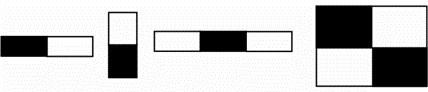
\includegraphics[height=0.1\textheight]{img/haar.jpg}
	\caption{Признаки Хаара}
    \label{img:haar}
    \end{figure}

    Значение каждого признака вычисляется по следующей формуле:

    \begin{equation}
        F = X - Y,
    \end{equation}

    где X - сумма интенсивностей пикселей, находящихся в светлой области признака, Y - сумма интенсивностей пикселей, находящихся в темной области признака.

    Для вычисления данных сумм интенсивностей пикселей за константное время используется интегральное представление изображения.
    
    \item Алгоритм AdaBoost

    Для прогнозирования категории, к которой относится входной объект, в машинном обучении используется модель, называемая классификатором ~\cite{classifier}. Слабый (или простой) классификатор —-- это классификатор, который решающий задачу классификации чуть лучше, чем случайное угадывание ~\cite{weak}, т. е. вероятность ошибки меньше 50\%. 

    Для повышения точности аналитических моделей используется бустинг (англ. boosting) --- последовательная композиция алгоритмов машинного обучения, в которой каждый следующий алгоритм стремится компенсировать недостатки композиции всех предыдущих алгоритмов ~\cite{tomsk}. 
    В методе Виолы---Джонса в качестве бустинга выбран алгоритм AdaBoost, в ходе выполнения которого формируется сложный классификатор, состоящий из набора простых и имеющий меньшую вероятность ошибки, чем у каждого слабого классификатора по отдельности:

    \begin{equation}
        a_s(x) = \sum_{i=1}^{n}b_i * a_i(x),
    \end{equation}

    где x --- изображение, $a_s(x)$ --- сложный классификатор, $a_i(x)$ --- слабый классификатор, $b_i$ --- весовой коэффициент соответствующего слабого классификатора.

    Основные этапы работы алгоритма AdaBoost ~\cite{viola}:

    \begin{itemize}
        \item Инициализация весов объектов обучающего набора одинаковым значением;
        \item Для каждой итерации алгоритма на основе сравнения ошибок классификации выбирается слабый классификатор, который наилучшим образом разделяет обучающий набор с учетом текущих весов объектов;
        \item Для каждого выбранного классификатора вычисляется его ошибка и вес, отражающий точность разделения объектов;
        \item Обновление весов объектов таким образом, чтобы неправильно классифицированые объекты получили больший вес на следующей итерации;
        \item Формирование сложного классификатора на основе слабых классификаторов и их весов.
    \end{itemize}
    
    Таким образом, в ходе выполнения данного алгоритма путем исключения большинства имеющихся признаков выбираются наиболее подходящие для конкретного объекта, в результате чего формируется классификатор с критическими признаками.

    В качестве классификаторов в методе Виолы---Джонса используются вышеописанные признаки Хаара. Для каждого признака выбирается соответствующий порог для бинарной классификации объектов, т. е. для определения того, какие значения признака считаются положительными, а какие --- отрицательными. Выбор оптимального порога осуществляется таким образом, чтобы минимизировать ошибку классификации, учитывая веса объектов в процессе обучения алгоритма.
    
    \item Каскадная структура классификаторов - последовательное объединение усложняющихся классификаторов в каскадную структуру (рис.~\ref{img:cascade} ~\cite{astrahan}) ~\cite{viola}. Данная структура повышает скорость обнаружения объектов, фокусируя свою работу на наиболее информативных областях изображения ~\cite{tomsk}. Это достигается тем, что каскад пытается отсеять как можно больше отрицательных экземпляров на самом раннем этапе: количество вычисленных признаков для анализа отрицательных областей должно быть значительно меньше, чем количество признаков, вычисленных для положительных областей. Следовательно, более сложные классификаторы применяются только к тем областям, которые уже прошли отсев более простыми классификаторами, что экономит ресурсы и улучшает производительность системы.

    \begin{figure}[h]
	\centering
	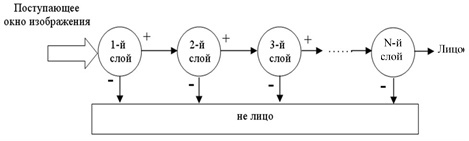
\includegraphics[width=120mm,height=0.17\textheight]{img/cascade.jpg}
	\caption{Каскадная структура классификаторов}
    \label{img:cascade}
    \end{figure}

    \item Сканирующее окно

    Для выделения областей, в которых могут находиться нужные объекты, используется сканирующее окно —-- перемещаемая прямоугольная активная область, в которой осуществляется поиск объектов ~\cite{tula}. Данный подход включает в себя пошаговый анализ различных прямоугольных подокон изображения, взятых с различными смещениями и масштабами. Впоследствии для каждой такой области применяются вышеописанные каскады классификаторов, которые оценивают, соответствует ли содержимое подокна определенным критериям.

\end{enumerate}

Алгоритм распознавания лиц:

\begin{enumerate}[label*=\arabic*.]
    \item Определить признаки Хаара.
    \item Сформировать обучающий набор и инициализировать веса объектов данного набора.
    \item Пока не достигнута заданная точность обучения:
    \begin{enumerate}
        \item Выбрать признак Хаара и порог, минимизирующие ошибку классификации при текущих весах.
        \item Вычислить вес полученного классификатора на основе ошибки классификации.
        \item Обновить веса объектов с учетом веса классификатора.
    \end{enumerate}
    \item Сформировать каскадную структуру из полученных классификаторов.
    \item Создать матрицу интегрального представления.
    \item Инициализировать сканирующее окно.
    \item Применить каскад классификаторов к текущему окну.
    \begin{enumerate}
        \item Если лицо обнаружено, то выделить эту область изображения, иначе продолжить проверку.
        \item Если не все окна проверены, то изменить параметры окна, иначе вернуть результаты обнаружения лиц.
    \end{enumerate}
\end{enumerate}
